\documentclass[a4j,titlepage,11pt]{jarticle}
\usepackage{thesis}
\usepackage[dvipdfmx]{graphicx}
\usepackage{amsmath}
\usepackage{bm}

\thesistype{卒業論文 or 修士論文} % "卒業論文" or "修士論文"
\title{日本語タイトル} % 日本語タイトル
\author{氏 名} % 氏 名
\date{令和4年1月25日} % 日付
\supervisor{氏 名} % 指導教員名
\supervisorposition{役職} % 指導教員の役職
\belonging{名城大学理工学部電気電子工学科 or 名城大学理工学研究科} % 所属

\begin{document}
\maketitle

% ↓ 修論は以下のコメントアウトを外してAbstractも書く
% \begin{abstract}

%   % ↑ 1行空ける
%   修論はAbstractも書く．
% \end{abstract}

% 目次
\TableOfContents

% 本文
\Section{はじめに}
背景，課題，目的を書く．

目的は課題を解決するうえで明らかにしたいことや実現したいことを指す．

問題と課題は混同しやすいので注意すること．
問題は目的を果たすうえで障害になっていることを指す．
課題は目的を果たすうえで実行すべきことである．
問題と課題の例を次に示す．
\begin{itemize}
  \item 問題 : 処理が遅い
  \item 課題 : 処理の高速化
\end{itemize}

\Section{関連研究}
課題を解決するために使えそうな世界クラスの研究を種類分けして解説する．
自分が勉強していることをアピールする．

\SubSection{種類分けの例}

\begin{itemize}
  \item DNNを使用/不使用
  \item カメラだけの手法/他センサ使用
\end{itemize}

\SubSection{解説内容}

\begin{itemize}
  \item 手法の概要 (世界はどんな工夫で課題を解決しようとしているか)
  \item 自分の課題に対して使えない理由
\end{itemize}

\Section{提案手法}

\SubSection{提案の概要}
アイデアの着想に至った経緯を書く．
アイデアの一番のポイントを1,2文で分かるように書く．

\SubSubSection{提案の詳細}
文字だけでなく，図や式を多用すること．
手法のメインアイデアとそれ以外の細かい内容は，節を分けて書くこと．

\SubSubSection{提案手法その1の具体的なこと2}
卒論を読んだ人が自分のシステムを作れるようにキーアイデア以外も細かく記載すること．

\SubSection{提案の概要2}

\SubSubSection{提案2の詳細1}

回転ベクトルを\Eq{Eq:1}に表す．すると回転量は\Eq{Eq:2}のように表され，単位ベクトルは\Eq{Eq:3}のように表される．

% 数式
\begin{equation}
  \bm{v} = \begin{bmatrix}
    v_{x} \\ v_{y} \\ v_{z}
  \end{bmatrix}
  \label{Eq:1} % 設定したラベルを使って \Eq{Eq:1} で本文から参照できる．
\end{equation}

\begin{equation}
  \theta = | \bm{v} | = \sqrt{v_{x}^{2} + v_{y}^{2} + v_{z}^{2}}
  \label{Eq:2} % 設定したラベルを使って \Eq{Eq:2} で本文から参照できる．
\end{equation}

\begin{equation}
  \overline{\bm{v}} = \begin{bmatrix}
    \overline{v_{x}} \\ \overline{v_{y}} \\ \overline{v_{z}}
  \end{bmatrix} = \frac{\bm{v}}{|\bm{v}|}
  \label{Eq:3} % 設定したラベルを使って \Eq{Eq:3} で本文から参照できる．
\end{equation}

この回転ベクトルは，\Eq{Eq:4}のロドリゲスの回転公式で回転行列に変換できる．

\begin{equation}
  \bm{R} = \begin{bmatrix}
    \cos{\theta} + \overline{v_{x}}^{2} (1 - \cos{\theta}) & \overline{v_{x}} \, \overline{v_{y}} (1 - \cos{\theta}) - \overline{v_{z}} \sin{\theta} & \overline{v_{x}} \, \overline{v_{z}} (1 - \cos{\theta}) + \overline{v_{y}} \sin{\theta} \\
    \overline{v_{y}} \, \overline{v_{x}} (1 - \cos{\theta}) + \overline{v_{z}} \sin{\theta} & \cos{\theta} + \overline{v_{y}}^{2} (1 - \cos{\theta}) & \overline{v_{y}} \, \overline{v_{z}} (1 - \cos{\theta}) - \overline{v_{x}} \sin{\theta} \\
    \overline{v_{z}} \, \overline{v_{x}} (1 - \cos{\theta}) - \overline{v_{y}} \sin{\theta} & \overline{v_{z}} \, \overline{v_{y}} (1 - \cos{\theta}) + \overline{v_{x}} \sin{\theta} & \cos{\theta} + \overline{v_{z}}^{2} (1 - \cos{\theta})
  \end{bmatrix}
  \label{Eq:4} % 設定したラベルを使って \Eq{Eq:4} で本文から参照できる．
\end{equation}

\SubSubSection{提案2の詳細2}

\Fig{Fig:1}，\Table{Table:1}を参照．

% 図の挿入
\begin{figure}[tb]
  \centering
  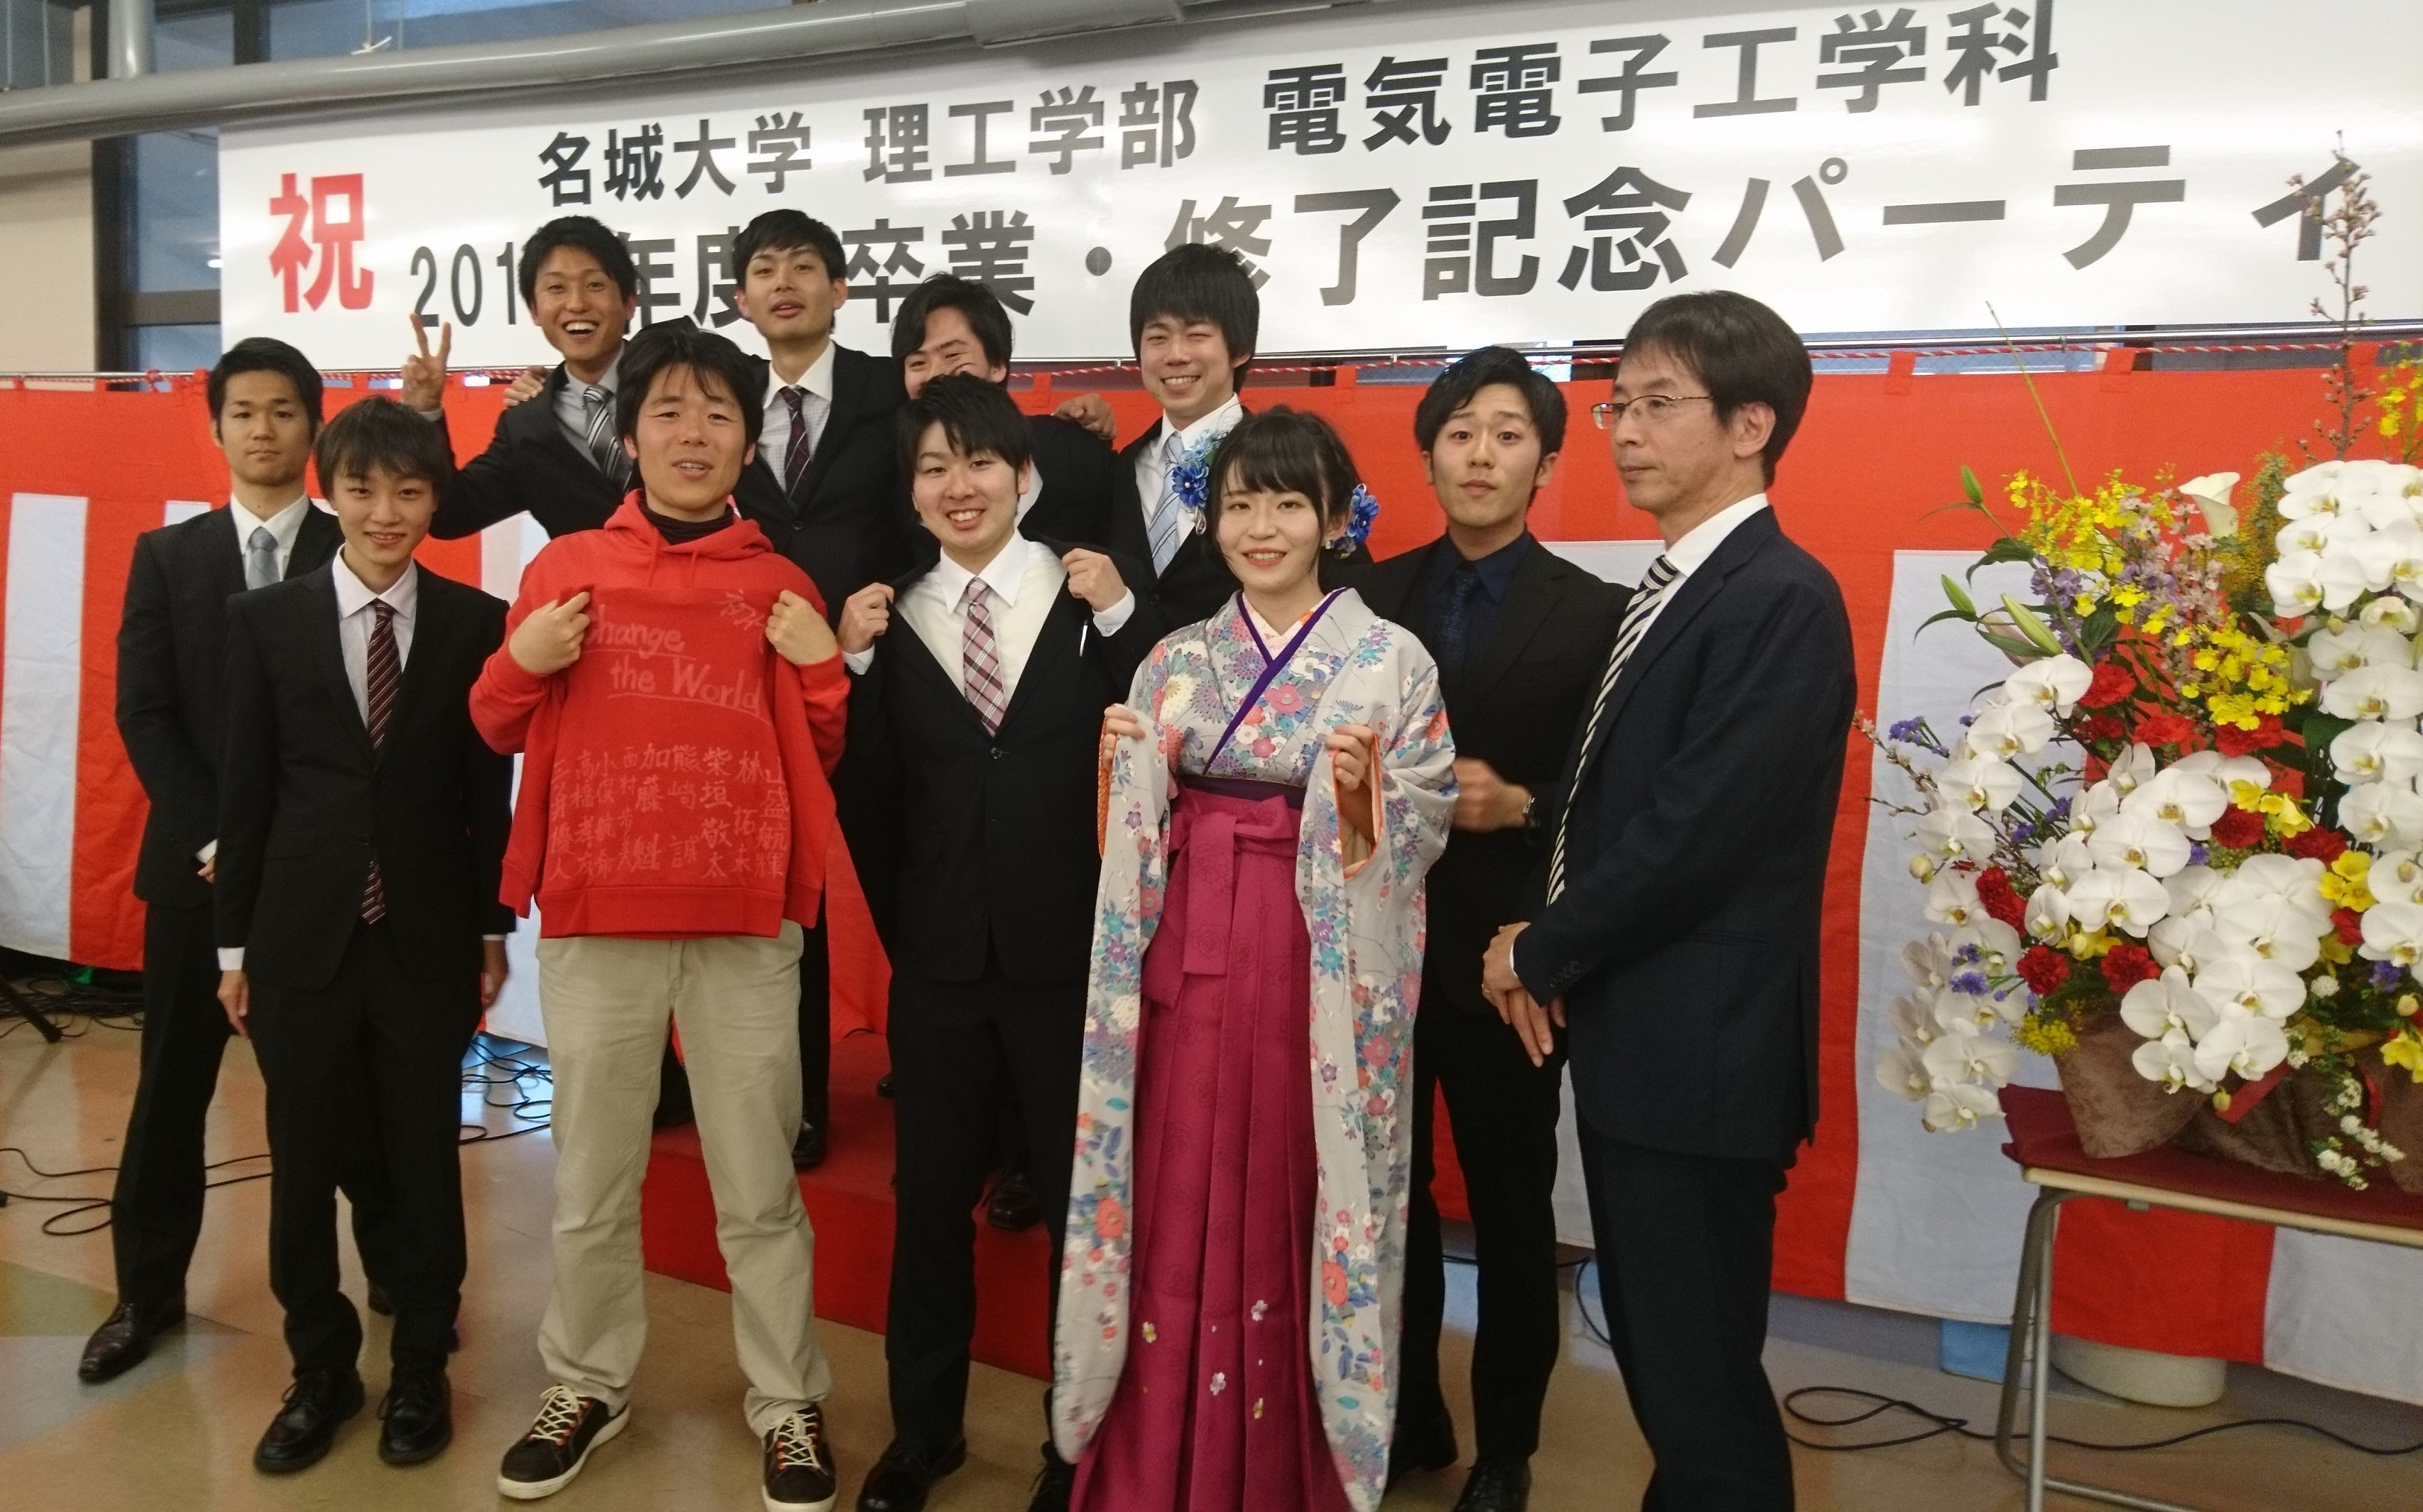
\includegraphics[width=\linewidth]{img/sample.jpg}
  \caption{田崎研究室 初代卒業生}
  \label{Fig:1} % 設定したラベルを使って \Fig{Fig:1} で本文から参照できる．
\end{figure}

% 表の挿入
% 
% 次のサイトが便利
% https://www.tablesgenerator.com/latex_tables
\begin{table}[tb]
  \centering
  \caption{研究室の所属人数の推移}
  \begin{tabular}{c|cccc}
    年度 & 2018 & 2019 & 2020 & 2021 \\ \hline
    B4 & $9$ & $8$ & $9$ & $8$ \\
    M1 & $0$ & $4$ & $5$ & $5$ \\
    M2 & $0$ & $0$ & $4$ & $5$ \\
  \end{tabular}
  \label{Table:1} % 設定したラベルを使って \Table{Table:1} で本文から参照できる．
\end{table}

\Section{評価実験}

実験が複数ある場合は，複数の節に分ける．

\SubSection{実験その1}

実験その1で何を確かめるのか，実験の目的を書いておくとよい．

\SubSubSection{実験環境}

ハードウェア構成として，ハードウェアの写真，型番，ブロック図などを書く．
ブロック図では各ブロックの入出力の内容を書いておく．

ソフトウェア構成として，ブロック図や各ブロックの入出力内容，使用したライブラリやそのバージョン，ソフトウェアのパラメータなどを記載する．

卒論を読んだ人が自分の実験結果を再現できるようにしておくこと．

\SubSubSection{実験設定}

\SubSubSection{実験結果および考察}

\SubSection{実験その2}

\SubSubSection{構成}

\SubSubSection{実験設定}

\SubSubSection{実験結果および考察}

\Section{おわりに}

\begin{itemize}
  \item 取り組んだ課題と目的
  \item 提案方法のキーアイデア
  \item 実験結果と分かったこと
  \item 今後の課題
\end{itemize}

% 謝辞
\begin{acknowledgement}
卒論や修論における謝辞とは，次のような方々に対して感謝の意を述べるためのもの．

\begin{enumerate}
  \item 卒論・修論の指導教官や副指導教官
  \item 指導教官以外でアドバイス・助言をいただいた先生
  \item 卒論・修論の研究に協力していただいた人・組織・企業など
\end{enumerate}

論文が完成するまでの間には，指導教官やゼミのメンバー，その他多くの方々の協力があったことだろう．その方々あるいは団体などにお礼を述べる場が「謝辞」というわけだ．
\end{acknowledgement}

% 参考文献
% reference.bib にbibtex形式で追加し，
% 本文中で\cite{}を使って参照すると自動的に追加される．
\Bibliography{reference}

% 付録
\SupplementBegin

実験内容を再現できるようにソフトウェアのインストール法や実行方法を具体的に書いておく．

\section{環境構築} % 付録の最初の章は"\section{}"を使う

\SubSection{ハードウェア構成}

\SubSection{Docker}

\Section{学習方法}

\end{document}
